%%%%%%%%%%%%%%%%%%%%%%%%%%%%%%%%%%%%%%%%%%%%%%%%%%%%%%%%%%%%%%%%%%%%%%%%%%%%%%
% Supplementary Information for:
% "An open-source, 3D-printed auger powder doser designed with generative
%  artificial intelligence" (Digital Discovery submission)
% Build: latexmk -pdf si.tex
%%%%%%%%%%%%%%%%%%%%%%%%%%%%%%%%%%%%%%%%%%%%%%%%%%%%%%%%%%%%%%%%%%%%%%%%%%%%%%
\documentclass[10pt]{article}
\usepackage[margin=2.2cm]{geometry}
\usepackage{graphicx}
\usepackage{booktabs}
\usepackage{longtable}
\usepackage{array}
\usepackage{hyperref}
\usepackage{mathptmx}

\renewcommand{\thetable}{S\arabic{table}}
\renewcommand{\thefigure}{S\arabic{figure}}
\renewcommand{\thesection}{S\arabic{section}}

\title{Supplementary Information\\[2mm]
\large An open-source, 3D-printed auger powder doser designed with generative
artificial intelligence}
\author{Sam Charles, Will Mulberry, Luke Winters, Carl Robinson,\\
Gage Erickson, and Sterling G. Baird}
\date{}

\begin{document}
\maketitle

\section{Bill of materials}

Table~\ref{tbl:bom} lists the parts for one channel, plus the items a platform
needs only once whatever its number of channels. Prices are single-unit US
dollars as of September 2026 and should be checked at order time; vendor links
are kept in \texttt{hardware/} in the repository
(\url{https://github.com/vertical-cloud-lab/powder-doser}).

\begin{table}[h]
\centering
\small
\caption{Bill of materials. Printed parts are excluded (about 260~g of PLA per
channel, under \$10), as are the custom circuit board, which can be replaced by a
breadboard, and the analytical balance (A\&D HR-100A, 0.1~mg readability),
which most laboratories already own.}
\label{tbl:bom}
\begin{tabular}{p{7.0cm}cp{1.4cm}p{4.0cm}}
\toprule
Part & Qty & Price (USD) & Source \\
\midrule
\multicolumn{4}{l}{\emph{Per channel}}\\
NEMA-11 bipolar stepper, 0.67~A, 10~N$\cdot$cm (11HS18-0674S) & 1 & 14 & StepperOnline \\
Pololu Tic T500 stepper controller & 1 & 33 & Pololu \#3135 \\
Pololu 33~V shunt regulator (clamps stepper back-voltage) & 1 & 15 & Pololu \#3776 \\
12~V push--pull solenoid, JF-0530B type (tapping) & 1 & 7.50 & Adafruit \#412 \\
DRV8871 H-bridge breakout (solenoid driver) & 1 & 7.50 & Adafruit \#3190 \\
ERM coin vibration motor, 10~mm & 1 & 1.95 & Adafruit \#1201 \\
DRV2605L haptic driver breakout (I$^2$C) & 1 & 7.95 & Adafruit \#2305 \\
MG996R-class metal-gear servo (tilt) & 2 & 24 & generic \\
Fasteners (M3), bulk capacitors & --- & 5 & generic \\
\midrule
\multicolumn{4}{l}{\emph{Shared (one per platform)}}\\
Raspberry Pi Pico~W & 1 & 6 & Raspberry Pi \\
Waveshare Pico-2CH-RS232 board (balance interface) & 1 & 9 & Waveshare 19979 \\
Mean Well GST60A12-P1J 12~V/5~A supply, cord and pigtail & 1 & 26 & Digi-Key \\
Pololu D24V22F5 5~V buck regulator & 1 & 19 & Pololu \#2858 \\
Headers and wiring & --- & 10 & generic \\
\midrule
\multicolumn{2}{l}{\textbf{Total, single-channel platform}} & \textbf{$\approx$185} & \\
\bottomrule
\end{tabular}
\end{table}

\section{Construction guide}

An illustrated build guide is kept in the repository alongside the parametric
CAD sources and STL files for every part. In outline:

\begin{enumerate}
\item \textbf{Print} the auger, the 20-tooth pinion, the bracket and collars,
the tap collar (two clamp halves), the mounting plate, the hinged baseplate and
the servo gear sector in PLA (0.2~mm layers, four perimeters, 25\% infill, no
supports). Print the auger upright.
\item \textbf{Auger drive:} seat the auger in its printed collars on the
mounting plate, bolt the NEMA-11 stepper with its pinion to the plate, and
check that the pinion meshes with the auger's 44-tooth gear band (2.2:1).
\item \textbf{Tap collar:} clamp the two collar halves around the auger tube,
mount the solenoid on the collar flange (2$\times$M3) so that its plunger
strikes the anvil pad, and stick the vibration motor to the opposite pad.
\item \textbf{Tilt stage:} join the mounting plate to the baseplate through the
side hinges (printed pins), mesh the two servos with the plate's gear (2:1), and
check that the outlet lies on the hinge axis.
\item \textbf{Electronics:} wire the Pico~W, Tic T500 (serial), DRV8871,
DRV2605L (I$^2$C), the RS-232 board (to the HR-100A balance) and the servos as
shown in the schematic in \texttt{hardware/test-module/}, then flash the
MicroPython firmware.
\item \textbf{Checkout:} run the firmware self-test (rotate, tap, vibrate,
tilt, tare and read), then the test protocols listed in the main text.
\end{enumerate}

\section{Auger and outlet geometry}

Fig.~\ref{fgr:nozzles} shows a cross-section of the geared auger and the four
printed outlet variants. The tests in the main text used the Type~4 outlet,
with a 3~mm exit hole.

\begin{figure}[h]
\centering
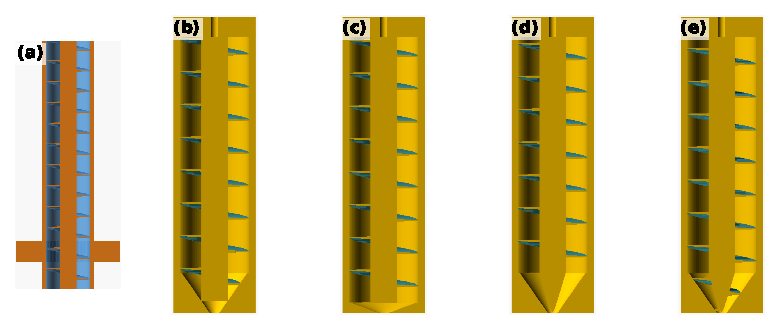
\includegraphics[width=0.95\textwidth]{figures/figS1_nozzles}
\caption{(a) Cross-section of the geared auger: the 8~mm central core, the
single-start helical flight (10~mm pitch, 2~mm thick) fused to the 21~mm bore of
the tube, and the external gear band. (b--e) Cross-sections of the four outlet
variants (Types~1--4), which differ in exit constriction and chamfer. All are
parametric OpenSCAD models (\texttt{cad/auger-geared/} in the repository)
written by AI coding agents under human review; no conventional CAD software was
used to design them.}
\label{fgr:nozzles}
\end{figure}

\section{Bench noise}

Protocol~A takes eight balance readings with nothing moving at the start of
every run. Their spread sets the smallest change that run can resolve
(Fig.~\ref{fgr:bench}). It was 0.0~mg on every run up to 12 August 2026 and
rose to tens of milligrams from 20 August. The cause was later traced to powder
trapped under a misaligned dust plate on the balance; after cleaning, the
balance drifted by less than 0.1~mg over 16 minutes. All data in the paper
predate that fix.

\begin{figure}[h]
\centering
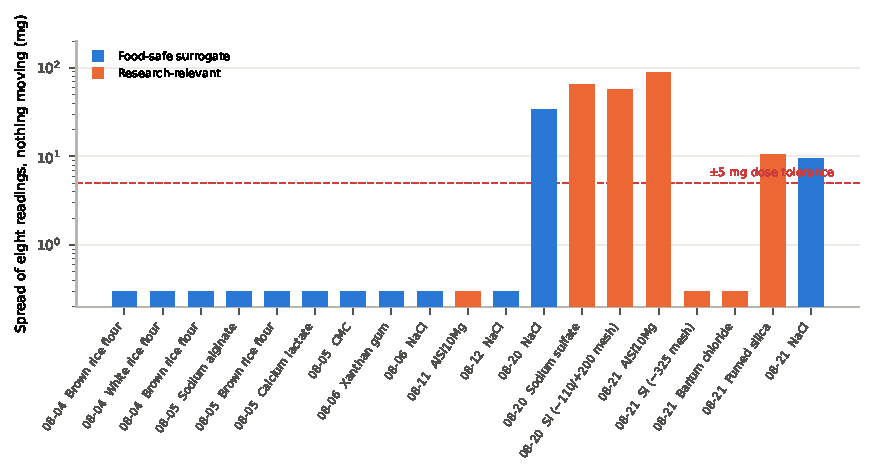
\includegraphics[width=0.95\textwidth]{figures/figS2_bench}
\caption{Balance noise floor for every first-round run: the spread (maximum
minus minimum) of eight readings taken with nothing moving (protocol~A), in
date order. Runs whose eight readings were identical are drawn at the axis
floor. The dashed line is the controller's $\pm$5~mg stopping band.}
\label{fgr:bench}
\end{figure}

\section{Closed-loop dose record}

Table~\ref{tbl:doses} summarizes every valid closed-loop dose by powder and
target mass. A dose is valid when its run passed quality screening, the dose
ended in a defined controller state, and the auger or solenoid actually moved;
doses excluded for any other reason (for example, a misaligned outlet, an
unreadable balance or powder that caked in the tube) are listed with the reason
in the per-dose file.

\small
% Generated by paper/figures/make_data_figures.py -- do not edit by hand.
\begin{longtable}{llcrrrccr}
\caption{Closed-loop dose summary for every valid dose (protocol G at 1~g; protocol H at 50 and 200~mg). Error is delivered minus requested mass. \emph{Within limit}: doses inside the acceptance limit ($\pm$10\% at 50~mg, $\pm$5\% at 200~mg and 1~g). \emph{Firmware ok}: doses the controller ended inside its own $\pm$5~mg stopping band. Round 1: August 2026, balance read on its stability flag; round 2: September 2026, bracketed readings. Per-dose records, including invalid doses and the reason each was excluded, are in \texttt{paper/figures/data/doses\_all.csv}.}\label{tbl:doses}\\
\toprule
Powder & Target & Round & $n$ & Mean error (mg) & SD (mg) & Within limit & Firmware ok & Median time (s) \\
\midrule\endfirsthead
\toprule
Powder & Target & Round & $n$ & Mean error (mg) & SD (mg) & Within limit & Firmware ok & Median time (s) \\
\midrule\endhead
AlSi10Mg & 50 mg & 2 & 3 & +21.5 & 26.7 & 1/3 & 1/3 & 15 \\
Si ($-$110/+200 mesh) & 50 mg & 2 & 2 & +1.1 & 4.8 & 2/2 & 2/2 & 18 \\
Sodium sulfate & 50 mg & 2 & 3 & +28.9 & 15.7 & 0/3 & 0/3 & 10 \\
Calcium lactate & 50 mg & 2 & 2 & +9.8 & 15.8 & 1/2 & 1/2 & 30 \\
Xanthan gum & 50 mg & 2 & 3 & +17.8 & 36.4 & 2/3 & 2/3 & 37 \\
NaCl & 50 mg & 2 & 3 & +4.2 & 4.8 & 2/3 & 2/3 & 17 \\
CMC & 50 mg & 2 & 3 & -2.2 & 2.4 & 3/3 & 3/3 & 211 \\
White rice flour & 50 mg & 2 & 3 & -4.7 & 0.6 & 3/3 & 3/3 & 136 \\
Sodium alginate & 50 mg & 2 & 3 & -19.6 & 8.3 & 0/3 & 0/3 & 561 \\
Si ($-$325 mesh) & 50 mg & 2 & 3 & -50.0 & 0.1 & 0/3 & 0/3 & 31 \\
\midrule
AlSi10Mg & 200 mg & 2 & 3 & -0.3 & 2.7 & 3/3 & 3/3 & 214 \\
Si ($-$110/+200 mesh) & 200 mg & 2 & 3 & +9.8 & 19.8 & 2/3 & 2/3 & 34 \\
Sodium sulfate & 200 mg & 2 & 3 & +10.8 & 17.7 & 2/3 & 1/3 & 30 \\
Calcium lactate & 200 mg & 2 & 3 & -16.5 & 16.6 & 2/3 & 1/3 & 464 \\
Xanthan gum & 200 mg & 2 & 3 & +2.9 & 0.6 & 3/3 & 3/3 & 89 \\
NaCl & 200 mg & 2 & 3 & +2.8 & 9.2 & 2/3 & 2/3 & 53 \\
CMC & 200 mg & 2 & 3 & -22.6 & 23.4 & 1/3 & 1/3 & 903 \\
White rice flour & 200 mg & 2 & 3 & -4.9 & 0.1 & 3/3 & 3/3 & 766 \\
Sodium alginate & 200 mg & 2 & 3 & -101.5 & 73.3 & 0/3 & 0/3 & 903 \\
Si ($-$325 mesh) & 200 mg & 2 & 3 & -199.7 & 0.5 & 0/3 & 0/3 & 31 \\
\midrule
AlSi10Mg & 1 g & 2 & 3 & +1.9 & 6.6 & 3/3 & 2/3 & 65 \\
Si ($-$110/+200 mesh) & 1 g & 2 & 3 & +0.2 & 2.8 & 3/3 & 3/3 & 128 \\
Sodium sulfate & 1 g & 2 & 3 & -4.2 & 1.1 & 3/3 & 3/3 & 86 \\
Calcium lactate & 1 g & 1 & 3 & -26.5 & 9.9 & 3/3 & 0/3 & 263 \\
Xanthan gum & 1 g & 1 & 3 & -32.9 & 9.6 & 3/3 & 0/3 & 193 \\
NaCl & 1 g & 1 & 6 & -1.9 & 5.3 & 6/6 & 5/6 & 186 \\
CMC & 1 g & 1 & 3 & -43.2 & 5.4 & 3/3 & 0/3 & 668 \\
White rice flour & 1 g & 1 & 3 & -137.9 & 23.5 & 0/3 & 0/3 & 822 \\
Sodium alginate & 1 g & 1 & 3 & -291.5 & 18.2 & 0/3 & 0/3 & 840 \\
Brown rice flour & 1 g & 1 & 3 & -999.1 & 0.9 & 0/3 & 0/3 & 7 \\
Si ($-$325 mesh) & 1 g & 1,2 & 6 & -999.5 & 0.7 & 0/6 & 0/6 & 8 \\
\bottomrule
\end{longtable}

\normalsize

\section{AI usage log}

In line with \textit{Digital Discovery}'s guidance on the use of LLMs, all AI
interactions are preserved publicly in the repository:

\begin{itemize}
\item \textbf{CAD and code generation:} every coding-agent session (GitHub
Copilot coding agent and Claude-family models, 2026) is recorded as a pull
request containing the prompt (issue text and review comments), the generated
CAD code, rendered views and the human review thread.
\item \textbf{Design reviews and literature queries:} Edison Scientific query
scripts, task identifiers, raw answers and extracted references are archived
with the corresponding branches; the consolidated bibliography, with the
verification status of each entry, is \texttt{paper/references\_validation.md}.
\item \textbf{Text-to-CAD evaluations:} CADSmith run artifacts and the Zoo
Design Studio (Zookeeper agent) session transcripts and notes are preserved on
their branches.
\item \textbf{Analysis and writing:} the data-analysis scripts behind every
figure, and the AI-drafted revisions of this manuscript, are in
\texttt{paper/} with their review threads.
\item \textbf{Qualitative observations:} the team's running journal of AI
behaviour, good and bad, is discussion~\#39 in the repository.
\end{itemize}

\end{document}
